%% 情報学群実験第3,4(C)用のレポートテンプレート
%
\documentclass[a4j,titlepage]{jarticle}
%% プリアンブルここから
\usepackage[dvipdfmx]{graphicx}
\usepackage{url}
\usepackage{comment}
%
\title{\huge 配達支援システム\\
		外部設計書}
\author{第2.0版\\
        ONO-Systems\\}
\date{\today}

%本文
\begin{document}
\maketitle

%目次
\tableofcontents
\clearpage

\section{目的}
現在,日本で行われている形態の宅配便サービスが開始し,約40年ほど経過しています.近年のECサイトの拡大に伴い,食料品や日用雑貨などを購入する利用者も増えており,ネットショッピングは特別な商品を買う場所ではなく,近所への買い物と似たような感覚で利用する人々が増えているため,宅配便の取扱個数はさらなる増加が予想されます\cite{ref1}.\\
\ \ \ その一方で,全体の取扱個数の中でも約2割ほどが再配達になっており,さらに約4割の利用者が「配達されることを知らなかった」という調査結果が国土交通省の調査により明らかになっています(図2).この2割にのぼる再配達を労働力に単純に換算すると年間約9万人もの労働力に相当するとも言われています.また,再配達によりトラックなどから排出される二酸化炭素によって,地球温暖化問題にも影響を与えています.さらに,再配達と宅配便の取扱個数の増加により,配達員の長時間労働などの問題が生じ,配達員の人手不足も深刻になっています\cite{ref1}.\\
\ \ \ 利用者側からすると商品が届いて不在票をもらう前に,利用者側から容易に配達員に受け取りの可否を連絡することは難しいです.\\
%=====================================
\ \ \ そこで,弊社では情報技術を駆使することにより宅配業務における配達員の負担を軽減し,消費者の利便性にも配慮した配達支援システムを提案します.
%=====================================

\section{システム概要}
ここでは,システムの機能概要を説明します.

\subsection{サブシステムの概要}
本システム内を構築するためのサブシステムの概要を以下に示します.

\subsubsection{位置情報通知サブシステム}
配達員が利用者の住所に近づいた場合またはトラックに荷物を運びこむ営業所の時点で,配達員の位置情報を受信できます.

\subsubsection{配達物の受け取り可否選択サブシステム}
利用者は配達物の受け取り可否を選択することができ,その選択結果は配達員に送信されます.

\subsubsection{音声読み上げサブシステム}
配達員は,受け取り可能な利用者の名前と住所を合成音声で読み上げさせることができます.

\subsubsection{受け取り可否の地図上表示サブシステム}
配達員は,受け取り可能な利用者の名前や住所,時間帯を地図上にプロットして色などから情報を判断することができます.

\subsection{サブシステムの詳細}
サブシステムの詳細を以下に示します.

\subsubsection{位置情報通知サブシステム}
入力:\\
出力:\\
処理:

\subsubsection{配達物の受け取り可否選択サブシステム}
入力:\\
出力:\\
処理:

\subsubsection{音声読み上げサブシステム}
入力:\\
出力:\\
処理:

\subsubsection{受け取り可否の地図上表示サブシステム}
入力:\\
出力:\\
処理:


\section{利用者インタフェース設計書}
ここでは,利用者が用いる際に使用するユーザインターフェースの設計を示します.

\subsection{画面遷移図}
あとは「社長」にまかせた...

\subsection{共有画面詳細}
ここでは配達支援システムの共有画面詳細について記します.

\subsubsection{ホーム画面}
図\ref{fig:login}は配達支援システムのホーム画面です.この画面はログインしていない状態でアプリを起動した時に表示されるます.また,この画面から「ログイン」,「アカウント作成」,「パスワードを忘れた場合」に遷移します.

\begin{figure}[htbp]
 \begin{center}
  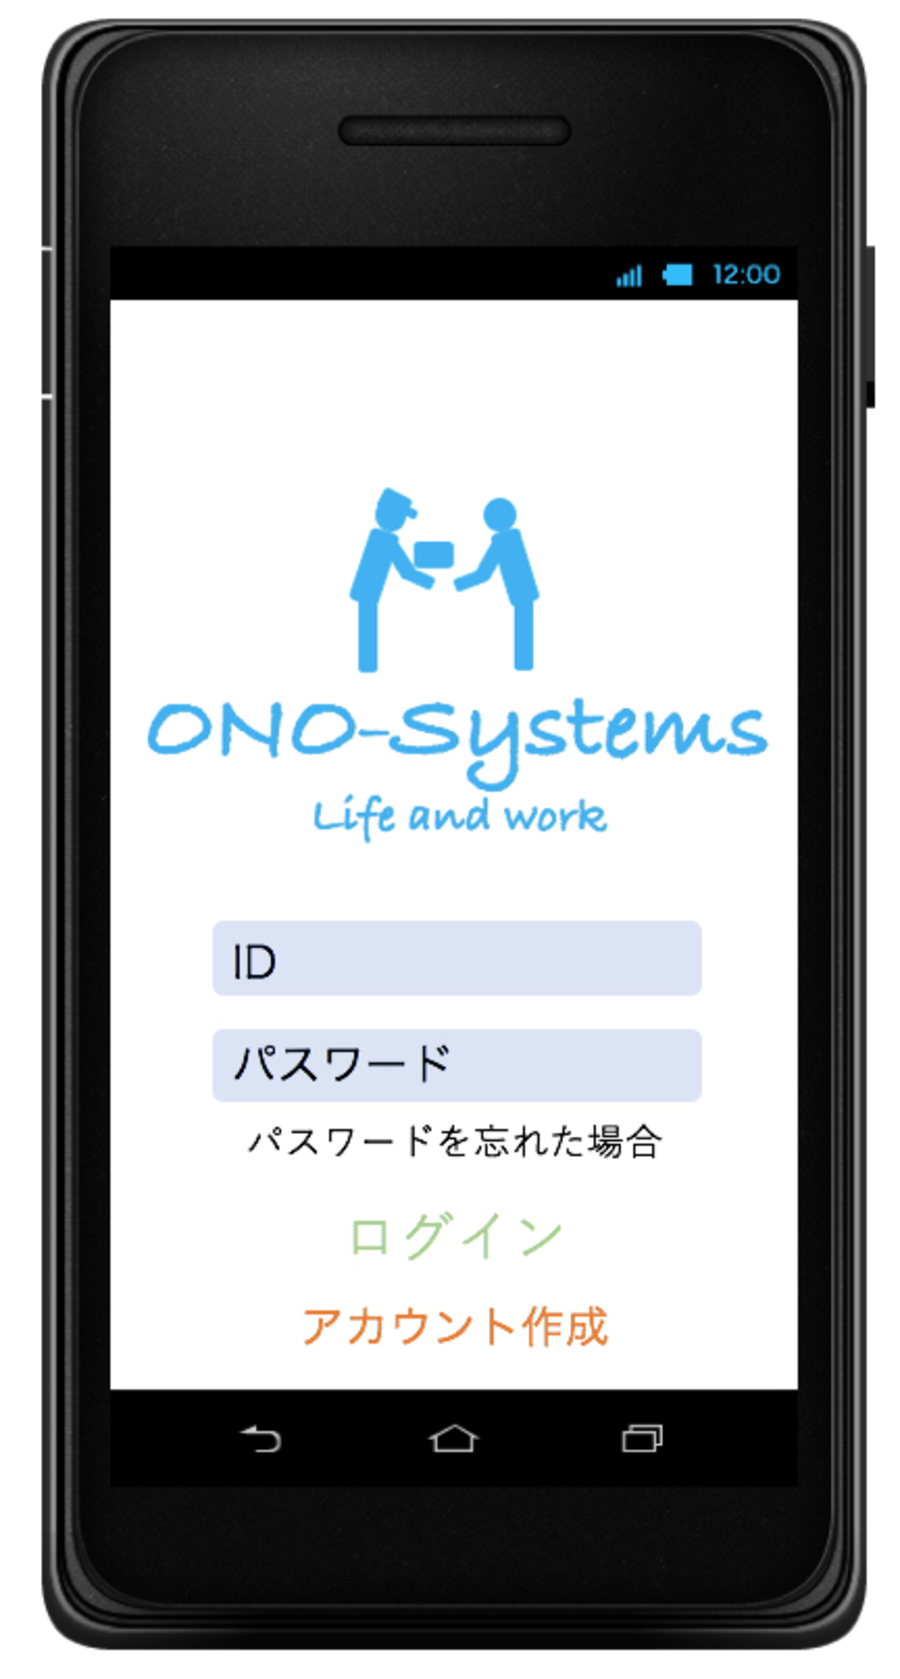
\includegraphics[width=50mm]{login.pdf}
	\caption{ログイン画面}
	\label{fig:login}
 \end{center}

\end{figure}


\subsubsection{パスワードを忘れた場合の画面}
図\ref{fig:ps_lost}は配達支援システムのパスワードを忘れた場合の画面です.この画面はホーム画面の「パスワードを忘れた場合」をタップすると表示されます.画面中央部の枠に既に登録してあるメールアドレスを入力し,送信をタップするとそのメールアドレスにパスワード再発行の為のURLが送られます.

\begin{figure}[htbp]
 \begin{center}
  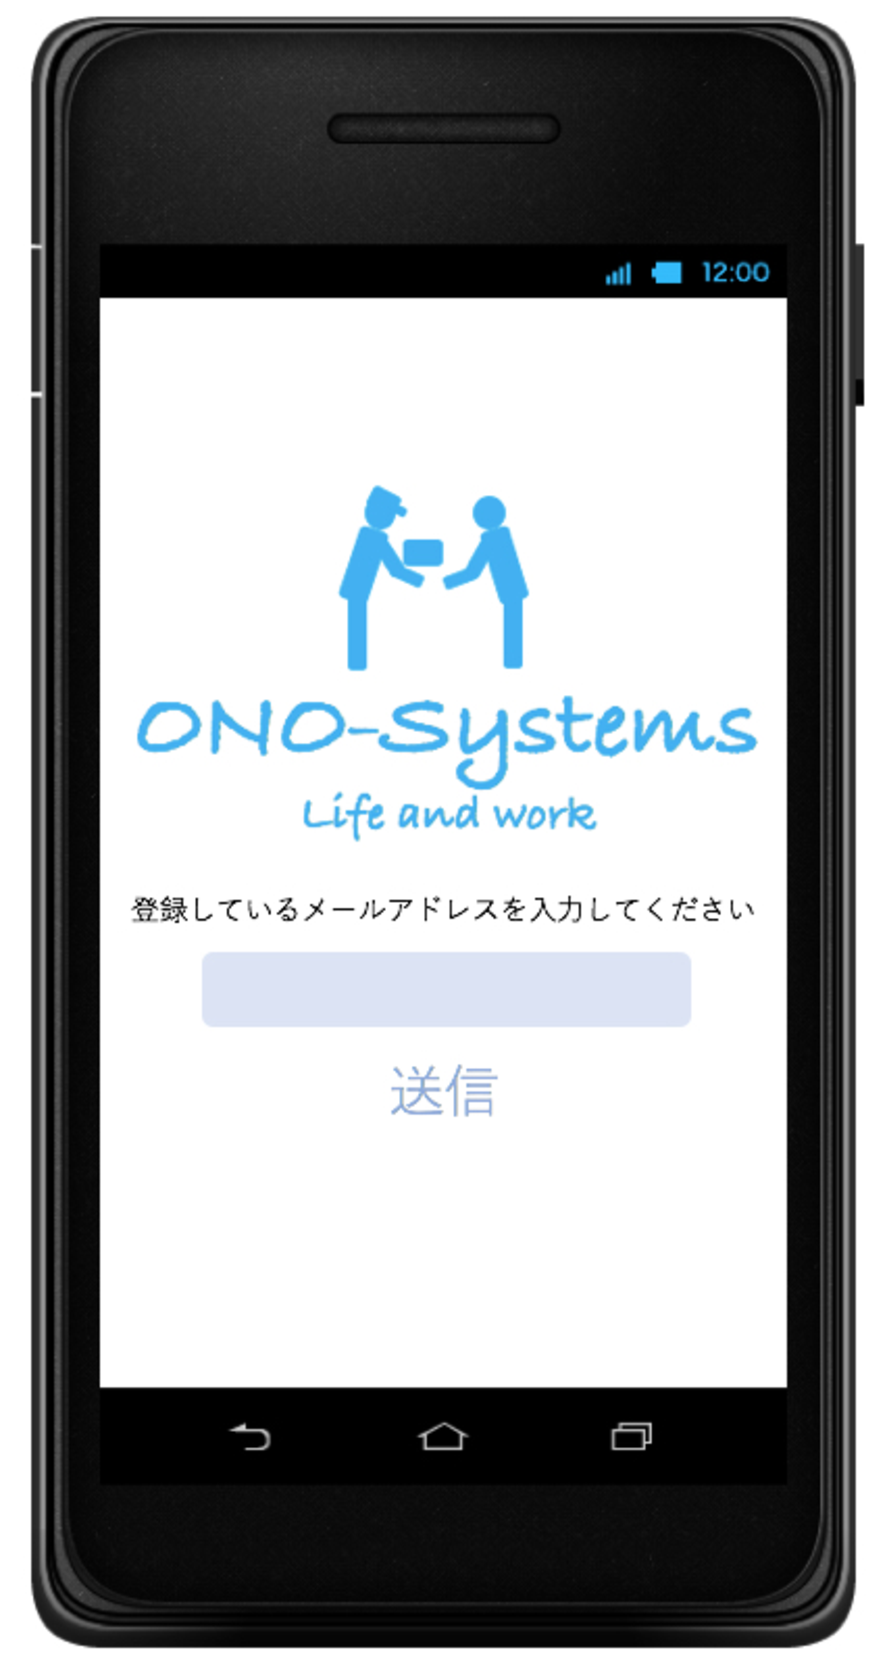
\includegraphics[width=50mm]{ps_lost.pdf}
	\caption{パスワードを忘れた場合の画面}
	\label{fig:ps_lost}
 \end{center}

\end{figure}

\subsubsection{パスワード再設定画面}
図\ref{fig:ps_change}は配達支援システムのパスワード再設定画面です.この画面は再発行の為のURLをタップすると表示されます.画面中央部の枠にパスワードを二回入力し,「パスワードの変更」をタップするとパスワード再発行が完了します.

\begin{figure}[htbp]
 \begin{center}
  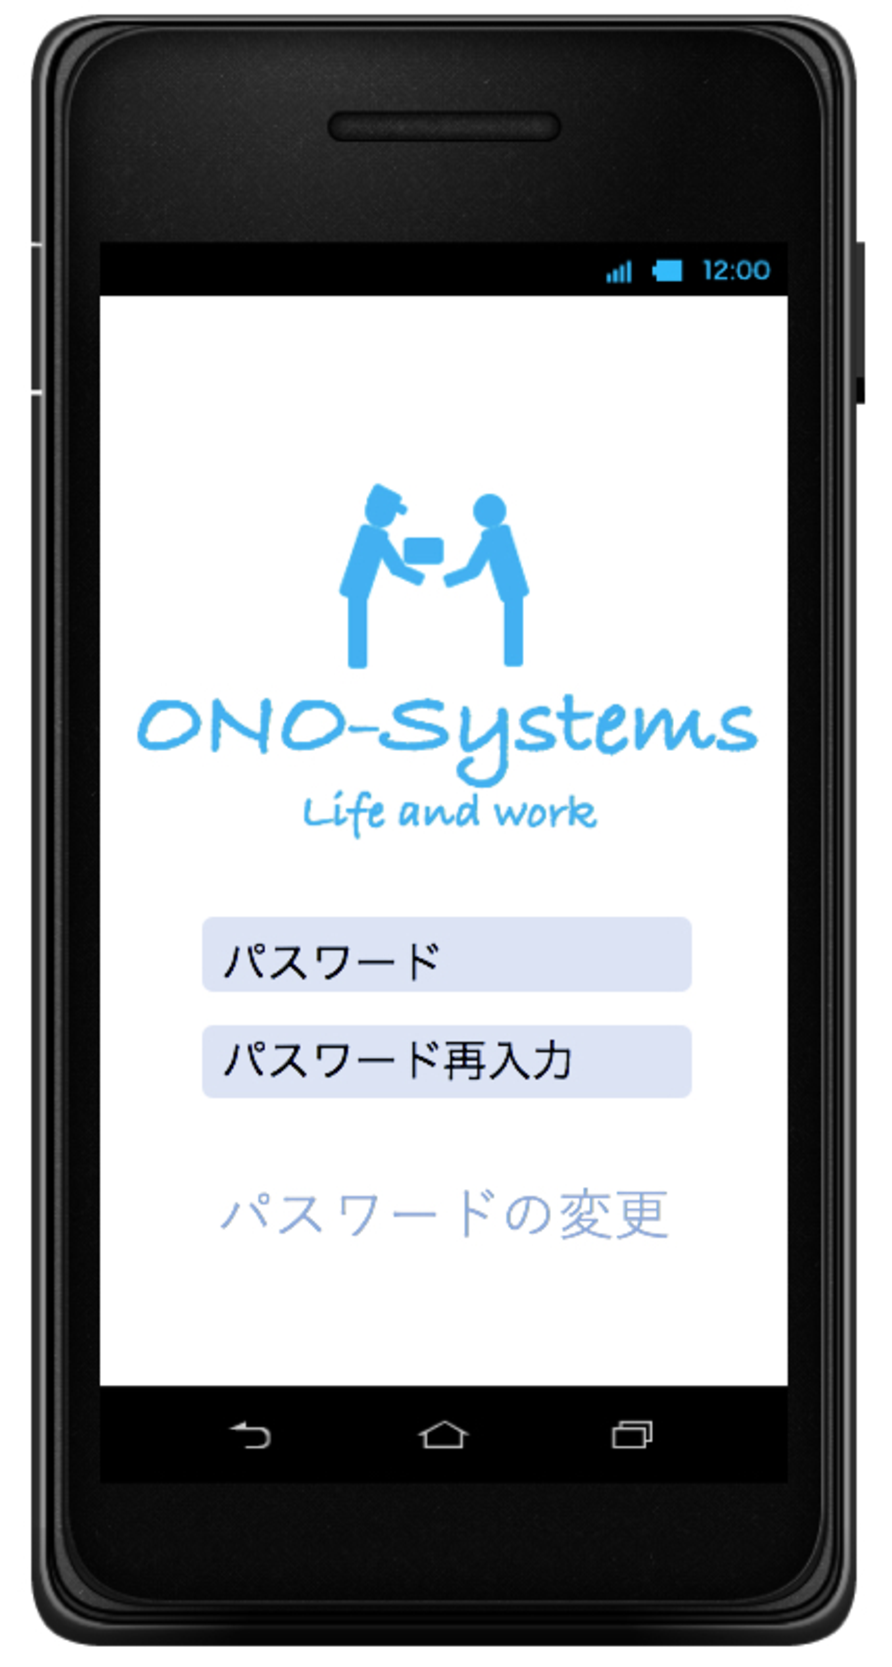
\includegraphics[width=50mm]{ps_change.pdf}
	\caption{パスワード再設定画面}
	\label{fig:ps_change}
 \end{center}

\end{figure}

\subsubsection{アカウント作成画面}
図\ref{fig:account_create}は配達支援システムのアカウント作成画面です.この画面はホーム画面の「アカウント作成」をタップすると表示されます.画面の入力欄に名前,メールアドレス,パスワード,パスワードの再入力,電話番号を入力し,「アカウント作成」をタップするとアカウントを作成することができます.アカウント作成後はユーザホーム画面に遷移します.

\begin{figure}[htbp]
 \begin{center}
  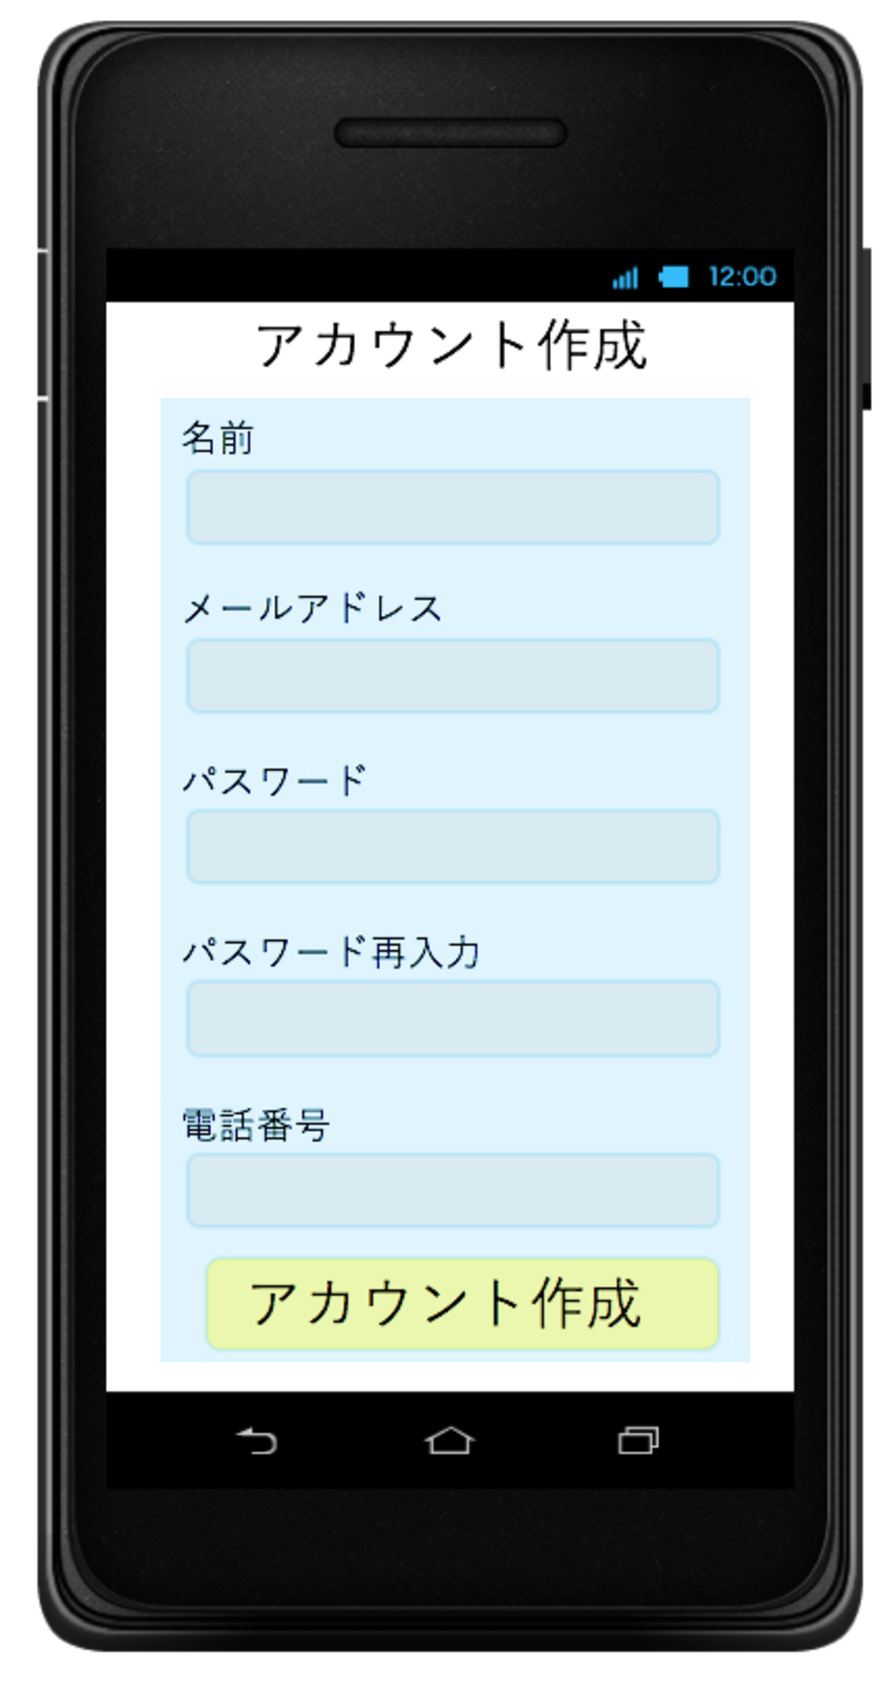
\includegraphics[width=50mm]{account_create.pdf}
	\caption{アカウント作成画面}
	\label{fig:account_create}
 \end{center}

\end{figure}

\subsection{ドライバー側画面詳細}
ここでは配達支援システムのドライバー側画面詳細について記します.

\subsubsection{ホーム画面}
図\ref{fig:driver_home}は配達支援システムのドライバーのホーム画面です.この画面はログイン画面でID,パスワードを入力し,ログインした場合に表示されます.また,既にログインしている場合はアプリ起動時に表示されます.この画面の機能は下記にて説明します.
\begin{enumerate}
	\item 利用者の選択結果のリアルタイム表示機能\\
	 \ 利用者の荷物受け取りの可否をリアルタイムに画面表示します.ドライバーが未読の間は各欄の左側に「new」と表示されます.
	\item ユーザ情報ボタン\\
	 \ ユーザのアカウント情報を表示,編集するサイドバーを出すことができます.
	\item 距離順ソートボタン\\
	 \ ドライバーから配達先までの距離を近い順にソートします.
	\item 時間順ソートボタン\\
   \ 時間指定の期限が短い順にソートします.
	\item 配達済みソートボタン\\
   \ 配達完了状態の荷物の表示・非表示を選択できます.
	\item 受け取り可否別表示ボタン\\
	 \ 「受け取れる」,「受け取れない」,「未選択」の三つを好きに表示・非表示できます.
	\item マップボタン\\
   \ マップ画面に遷移します.
	\item 検索バー\\
	 \ 入力された文字と一致する荷物を配達時間順(+距離?)に表示します.
\end{enumerate}

\begin{figure}[htbp]
 \begin{center}
  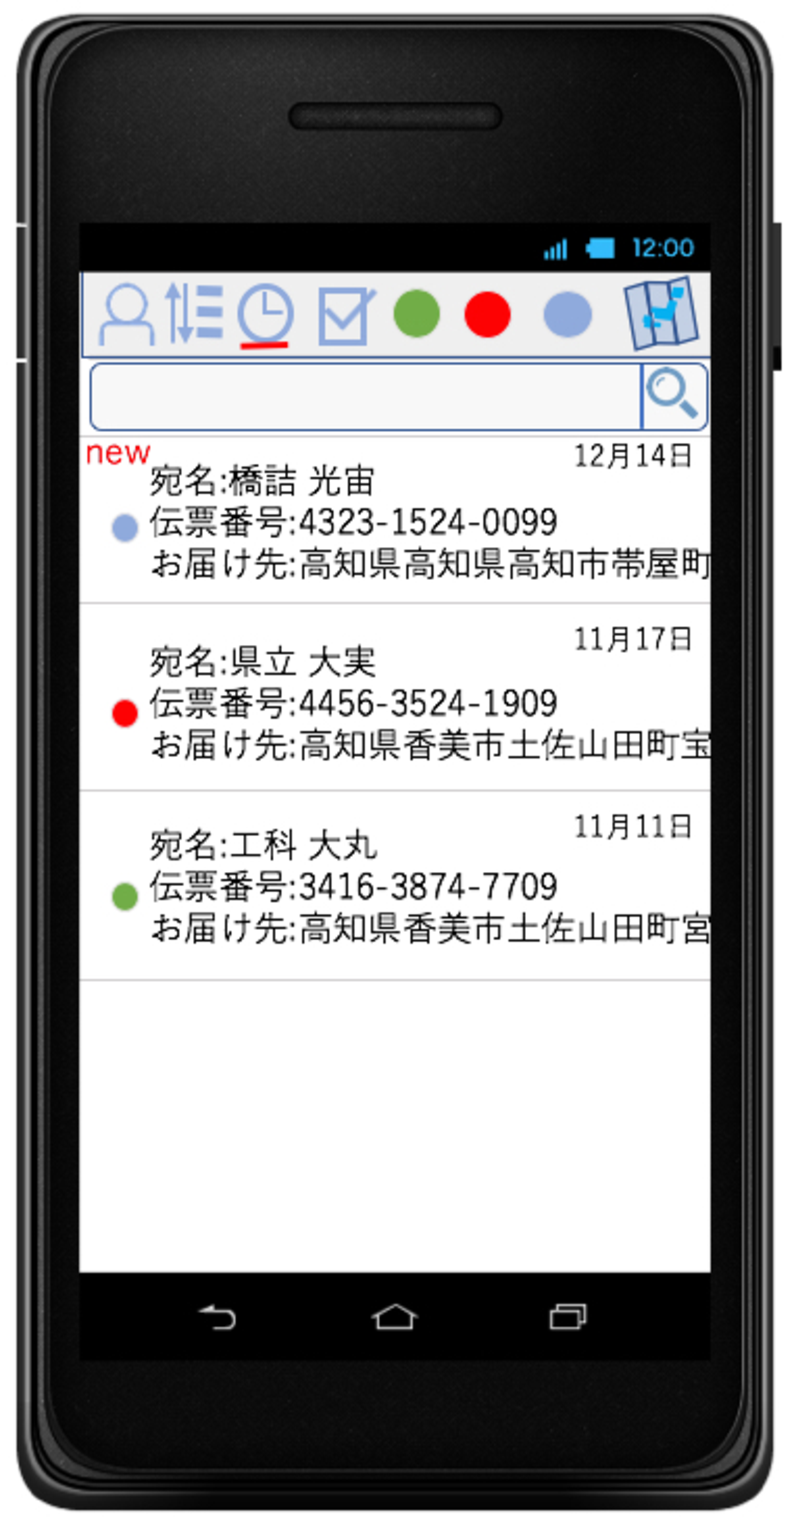
\includegraphics[width=50mm]{driver_home.pdf}
	\caption{ホーム画面}
	\label{fig:driver_home}
 \end{center}

\end{figure}




\subsubsection{サイドバー画面}
図\ref{fig:driver_side}は配達支援システムのサイドバーの画面です.この画面はホーム画面の「ユーザ情報ボタン」をタップすると表示されます.画面の各欄にはユーザの情報(名前,メールアドレス,パスワード,パスワード再入力,電話番号)が表示されており,変更したい部分を書き換えた後に更新ボタンを押すことでユーザ情報を変更することができます.また,画面中央上部の「×」ボタンまたはバックボタンをタップするとホーム画面に遷移します.

\begin{figure}[htbp]
 \begin{center}
  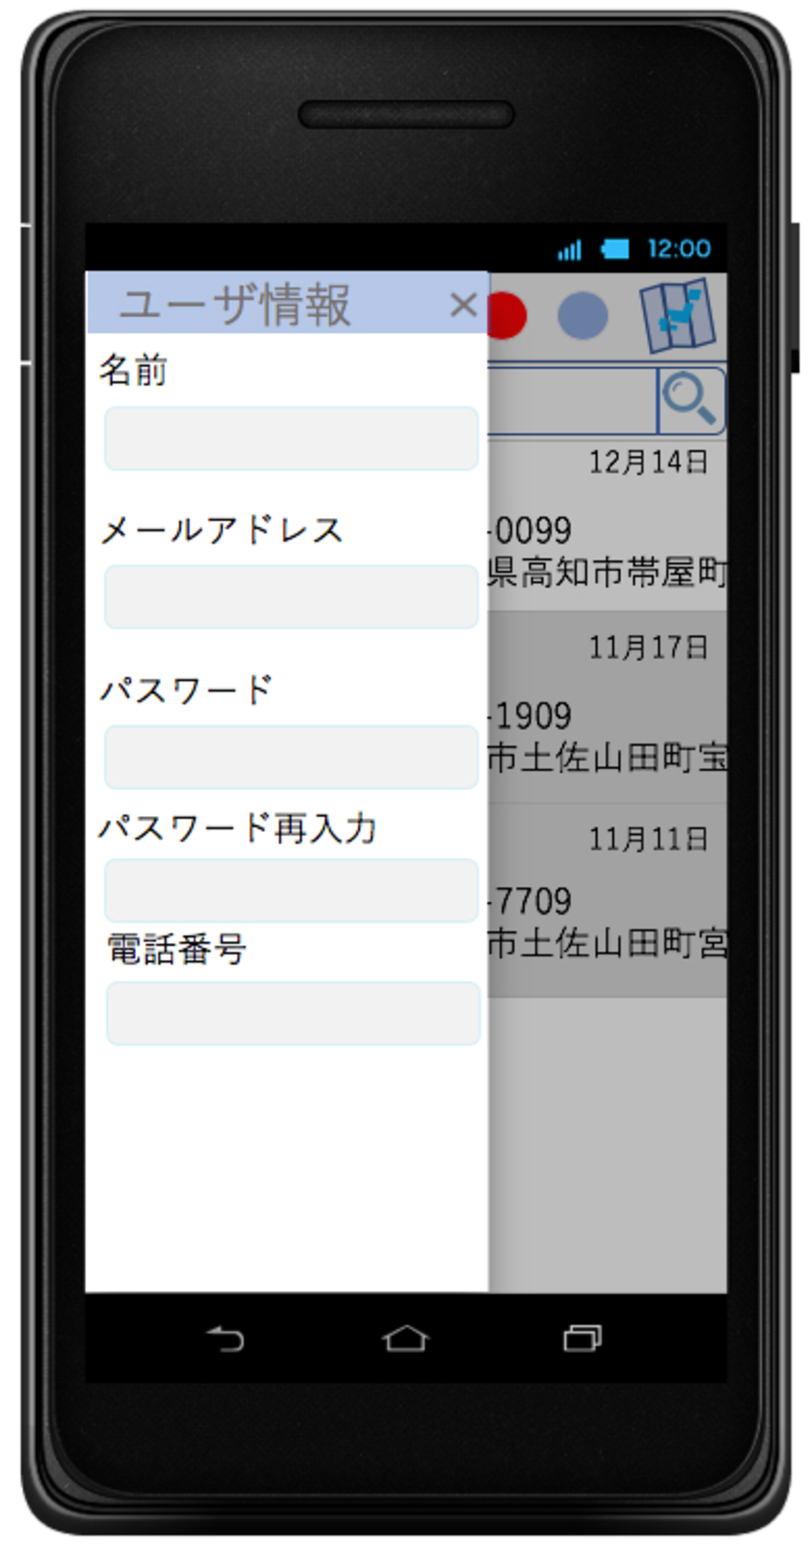
\includegraphics[width=50mm]{driver_side.pdf}
	\caption{サイド画面}
	\label{fig:driver_side}
 \end{center}

\end{figure}

\subsubsection{詳細画面}
図\ref{fig:driver_details}は配達支援システムの詳細画面です.この画面はホーム画面の各荷物欄をタップすると表示されます.画面には配達先の情報(宛名,伝票番号,住所,配達希望時間)が表示されており,プルダウン,更新ボタン,配達完了ボタン,マップボタンがあります.プルダウンでは配達希望時間を選ぶことができ,配達希望時間を変更した後に更新ボタンをタップすると配達希望時間を変更することができます.また,画面下の配達完了ボタンをタップすると配達完了状態にでき,画面右上のマップボタンをタップするとマップ画面へ遷移することができます.
\begin{figure}[htbp]
 \begin{center}
  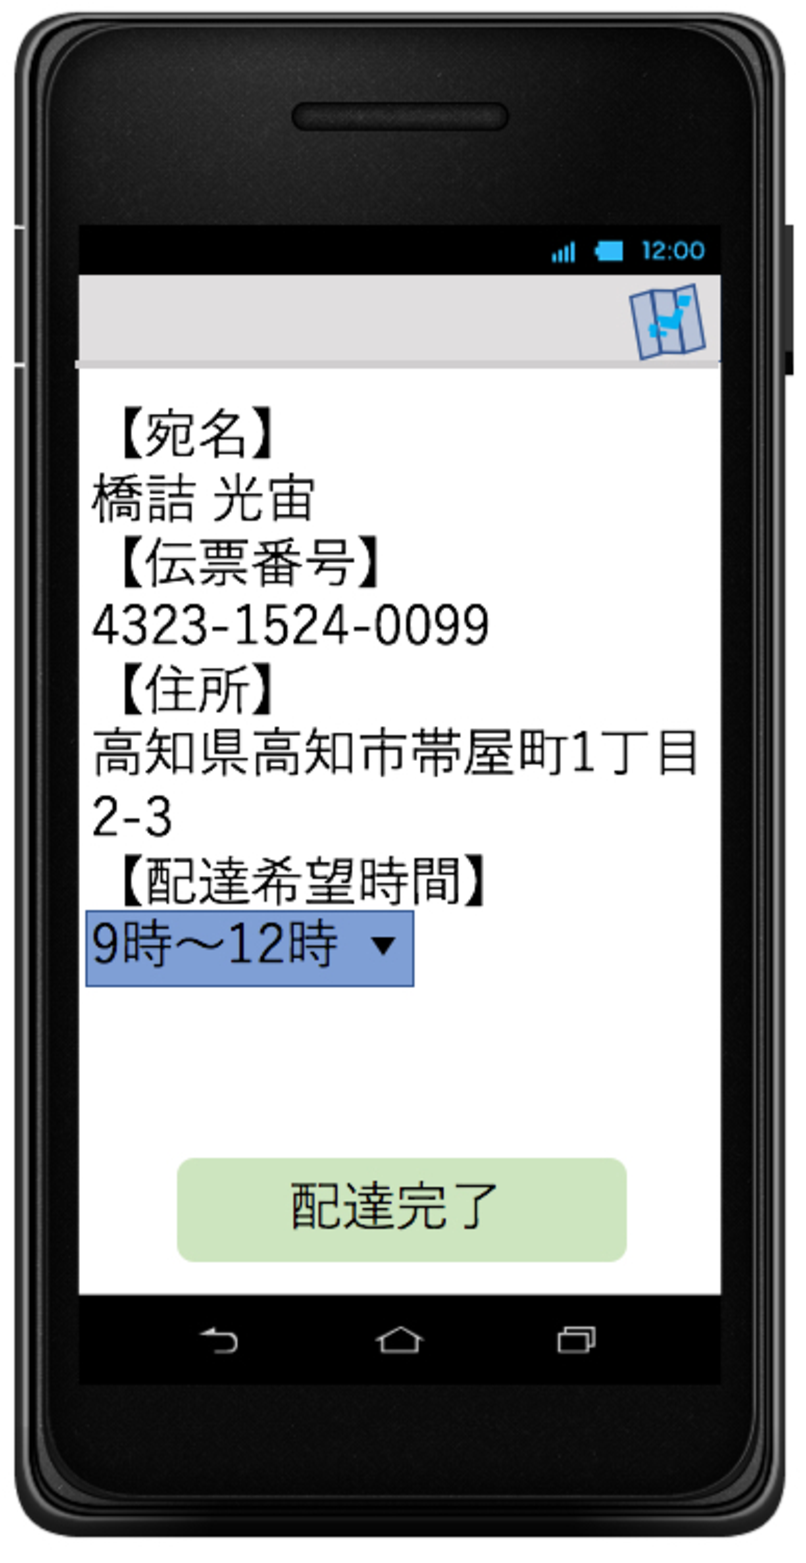
\includegraphics[width=50mm]{driver_details.pdf}
	\caption{詳細画面}
	\label{fig:driver_details}
 \end{center}

\end{figure}




\subsubsection{マップ画面}
図\ref{fig:map}は配達支援システムのマップ画面です.この画面はホーム画面,ドライバー詳細画面のマップボタンをタップすると表示されます.この画面の機能は下記で説明します.
\begin{enumerate}
	\item 配達先表示機能\\
	 \ 各ピンの場所に住所と配達指定時間が表示されます.下記で説明する絞り込み機能を使用している色は非表示になります.
	\item 受け取り可否表示機能\\
	 \ 各ピンの色で受け取りの可否を表示しています.赤が「受け取り不可」,緑が「受け取り可」,青が「未選択」を表しています.
	\item 絞り込み機能\\
   \ 不要な配達先表示を非表示にすることができます.

\end{enumerate}

\begin{figure}[htbp]
 \begin{center}
  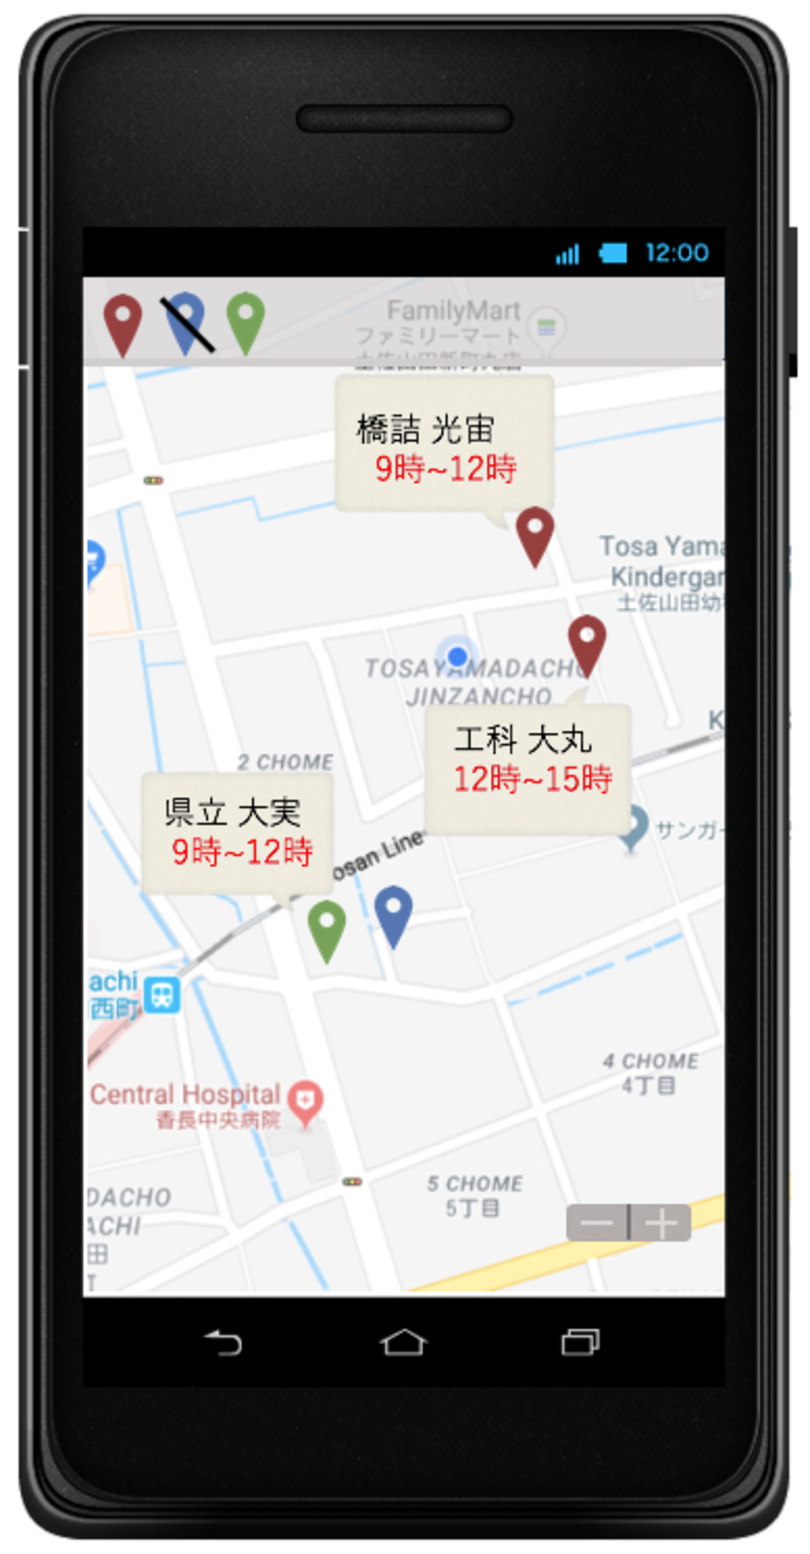
\includegraphics[width=50mm]{map.pdf}
	\caption{マップ画面}
	\label{fig:map}
 \end{center}

\end{figure}

\newpage

\subsection{ユーザ側詳細画面}
ここでは配達支援システムのユーザ側画面詳細について記します.

\subsubsection{ホーム画面}
図\ref{fig:user_home}は配達支援システムのドライバーのホーム画面です.この画面はログイン画面でID,パスワードを入力し,ログインした場合に表示されます.また,既にログインしている場合はアプリ起動時に表示されます.この画面の機能は下記にて説明します.
\begin{enumerate}
	\item 荷物の詳細確認機能\\
	 \ 画面に商品の詳細(商品名,伝票番号,お届け先,お届け日時)を表示しており,荷物を受け取るボタンと日時変更ボタンがあります.荷物を受け取るボタンをタップすると,ドライバーにに網を受け取る通知を送ります.日時変更ボタンをタップすると日時変更画面に遷移します.
	\item ユーザ情報ボタン\\
	 \ ユーザのアカウント情報を表示・編集するサイドバーを出すことができます.

	\item 配達済みソートボタン\\
   \ 配達完了状態の荷物の表示・非表示を選択できます.

	\item 受け取り可否別表示ボタン\\
	 \ 「受け取れる」,「受け取れない」,「未選択」の三つを好きに表示・非表示できます.

	\item 検索バー\\
	 \ 入力された文字と一致する荷物を配達時間順(+距離?)に表示します.

\end{enumerate}

\begin{figure}[htbp]
 \begin{center}
  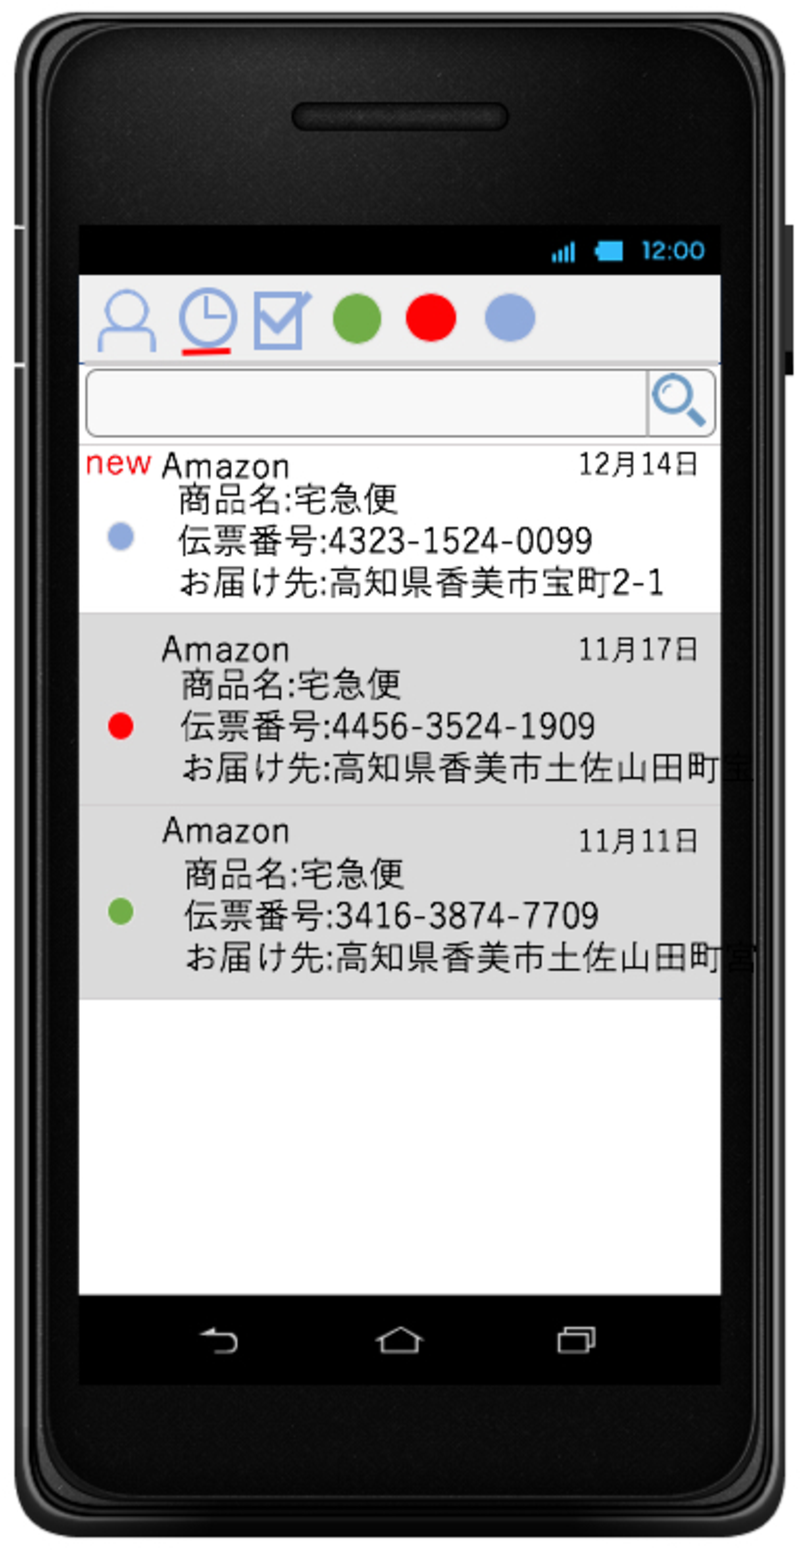
\includegraphics[width=50mm]{user_home.pdf}
	\caption{ホーム画面}
	\label{fig:user_home}
 \end{center}

\end{figure}

\subsubsection{サイドバー画面}
図\ref{fig:user_side}は配達支援システムのサイドバーの画面です.この画面はホーム画面の「ユーザ情報ボタン」をタップすると表示されます.画面の各欄にはユーザの情報(名前,メールアドレス,パスワード,パスワード再入力,電話番号,住所)が表示されており,変更したい部分を書き換えた後に更新ボタンを押すことでユーザ情報を変更することができます.また,画面中央上部の「×」ボタンまたはバックボタンをタップするとホーム画面に遷移します.

\begin{figure}[htbp]
 \begin{center}
  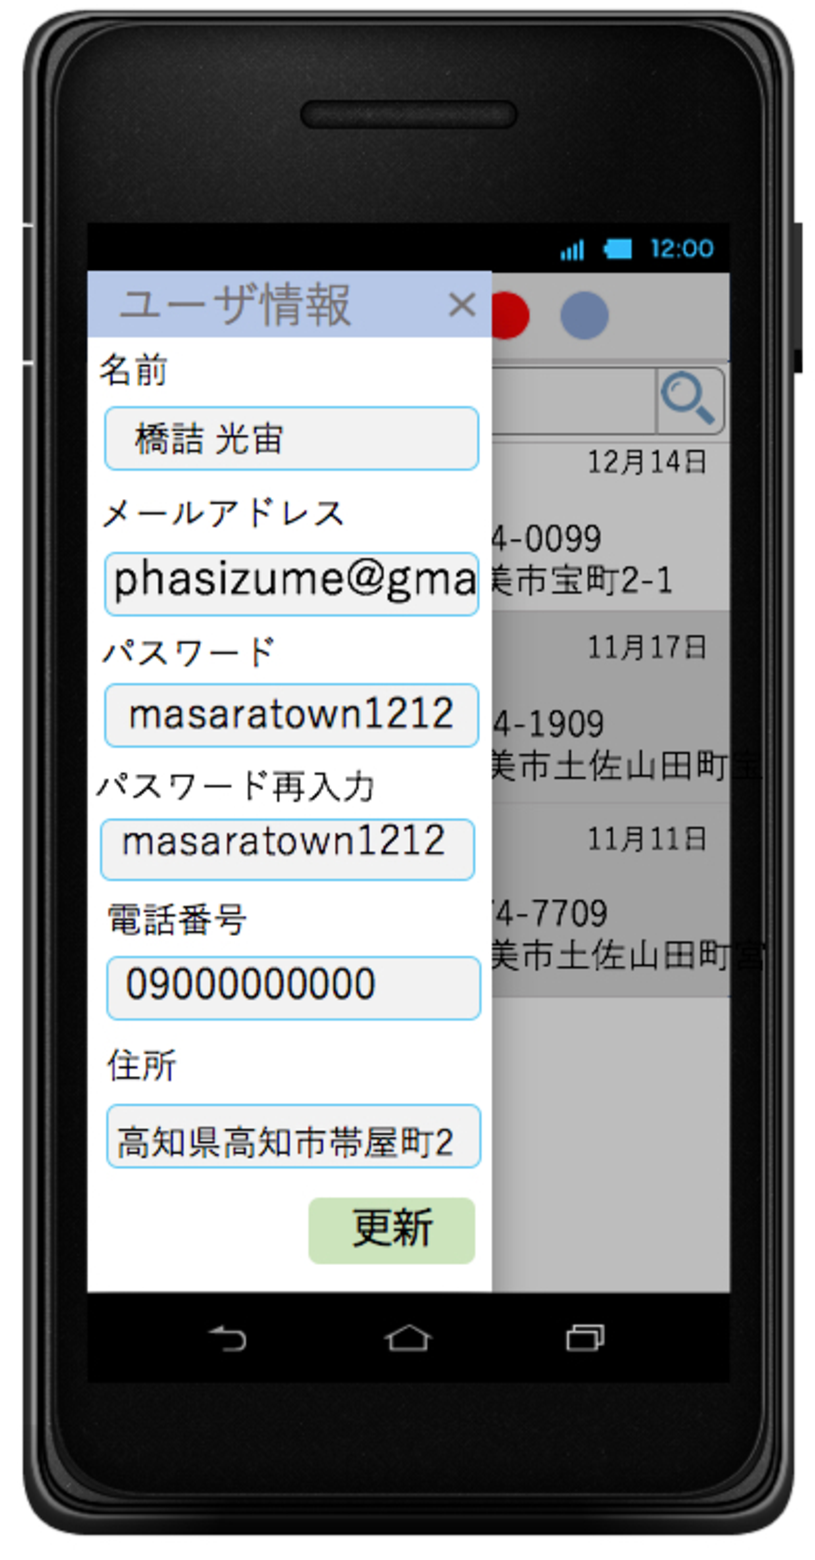
\includegraphics[width=50mm]{user_side.pdf}
	\caption{サイド画面}
	\label{fig:user_side}
 \end{center}

\end{figure}

\subsubsection{詳細画面}
図\ref{fig:user_details}は配達支援システムのユーザ詳細画面です.この画面はホーム画面の各荷物欄をタップすると表示され,画面には商品の情報(商品名,伝票番号,お届け先,お届け日時)が表示されます.画面下の「荷物を受け取る」をタップすると配達員に荷物を受け取れると通知され,ユーザホーム画面に遷移します.また,日時変更をタップすると時間変更画面に遷移します.
\begin{figure}[htbp]
 \begin{center}
  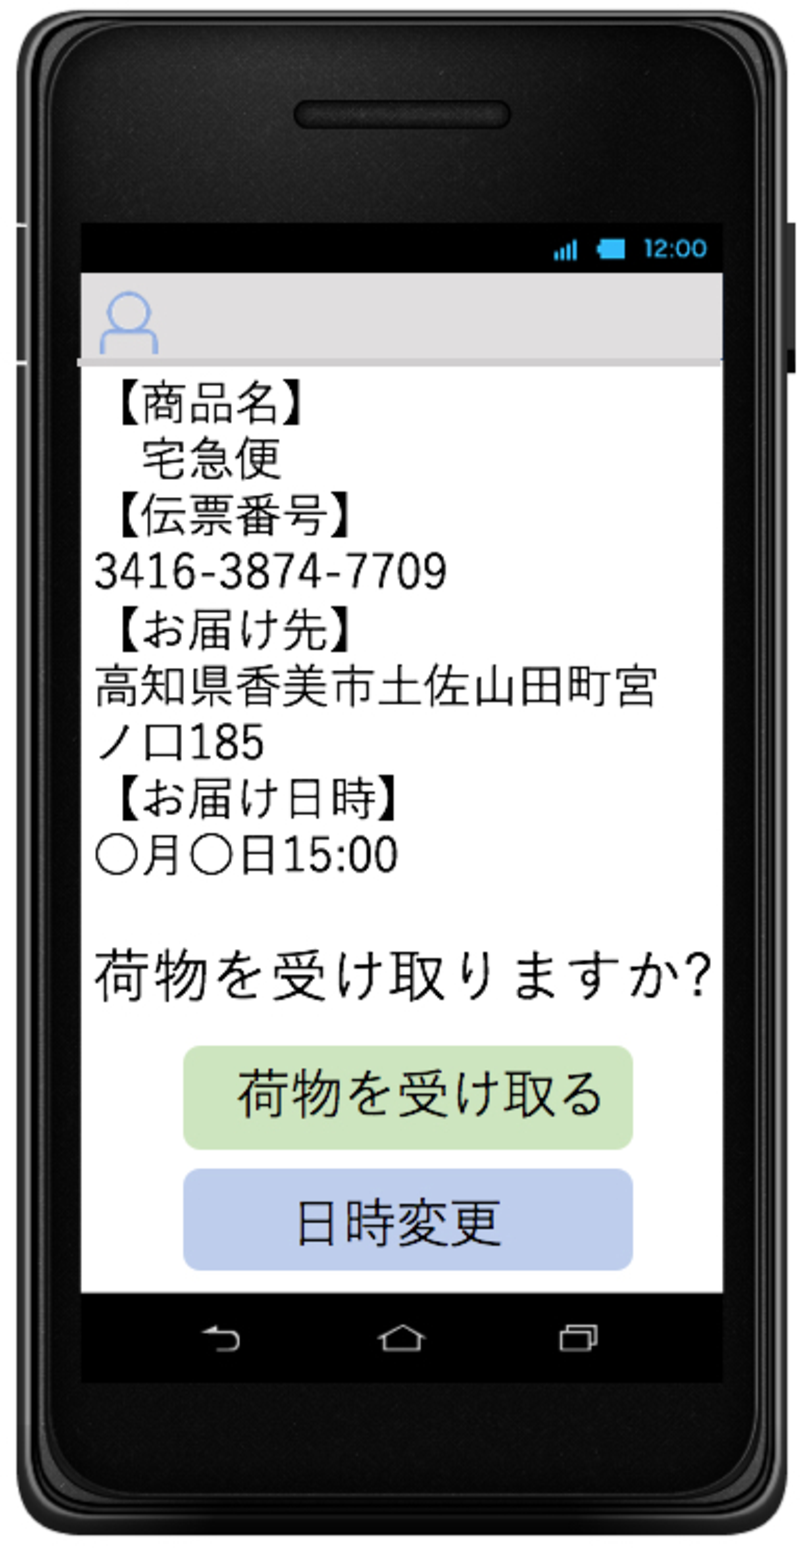
\includegraphics[width=50mm]{user_details.pdf}
	\caption{詳細画面}
	\label{fig:user_details}
 \end{center}

\end{figure}

\subsubsection{日時変更画面}
図\ref{fig:time_change}は配達支援システムの日時変更画面です.この画面はユーザ詳細画面の「日時変更」をタップすると表示され,画面には商品の情報(商品名,伝票番号,お届け先,お届け日時)が表示されています.「○月○日15:00お届け予定」の下をタップした後に日時を変更し,「変更確定」をタップすることで配達日時を変更できます.「変更確定」タップ後はユーザホーム画面に遷移します.

\begin{figure}[htbp]
 \begin{center}
  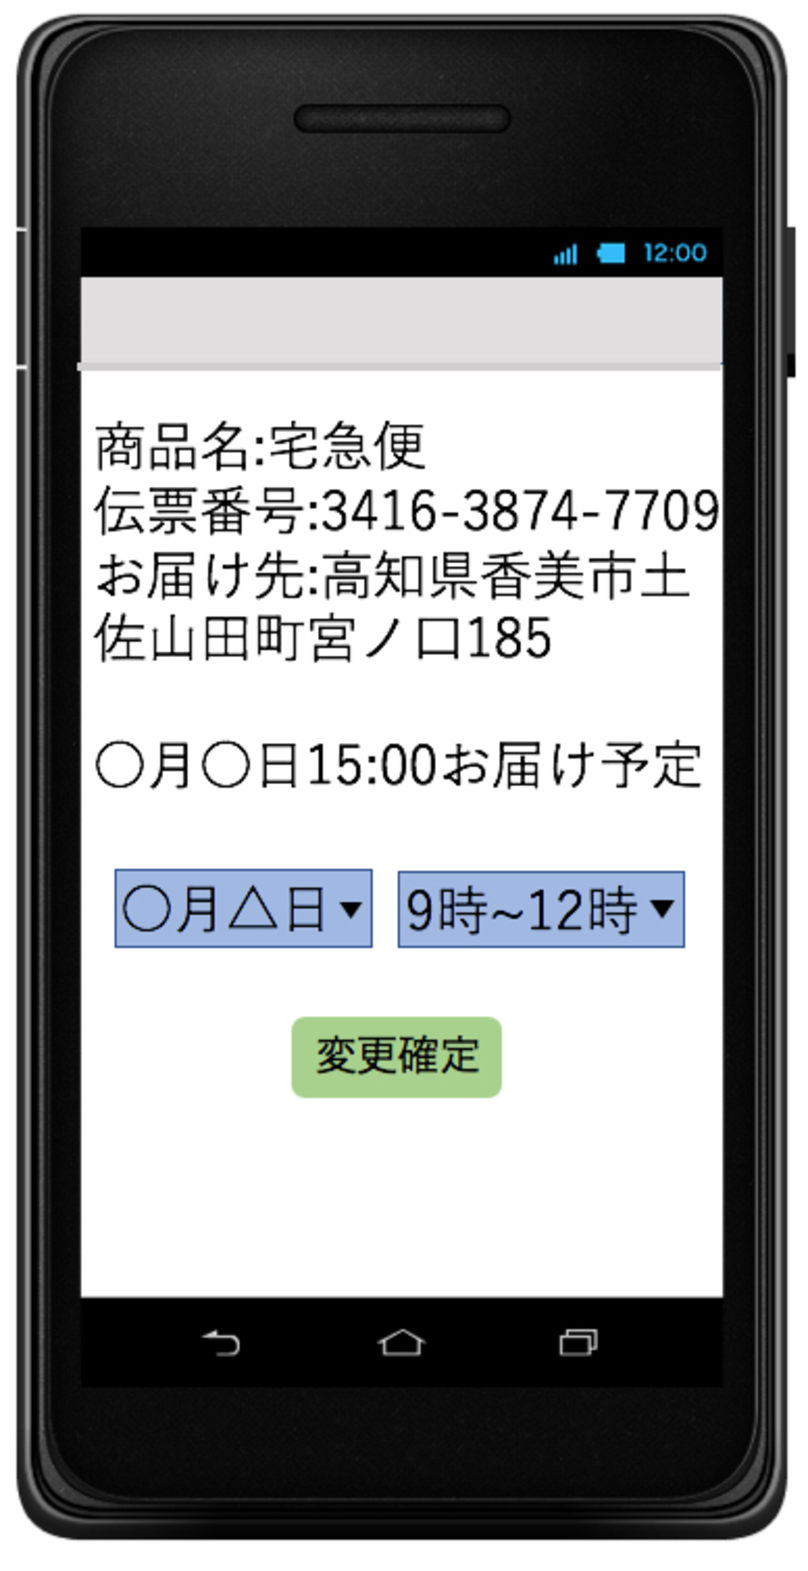
\includegraphics[width=50mm]{time_change.pdf}
	\caption{時間変更画面}
	\label{fig:time_change}
 \end{center}

\end{figure}

\section{システムのハードウェア構成}
本システムのハードウェア構成は表1の通りです.
\begin{table}[htbp]
\begin{center}
 \caption{ハードウェア構成}
  \begin{tabular}{|c|c|c|}\hline
    項目 & 数量 & 備考\\ \hline \hline
    サーバ & 1台 & AWS\\ \hline
    管理者端末 & 1台 & \\ \hline
  \end{tabular}
\end{center}
\end{table}


\section{ソフトウェア構成}
システム間のやり取りは,Java,MySQLを用いて行います.

\section{データベース設計}
本システムのデータベースには,4個のデータテーブルを用いる.各データテーブルの情報を以下に示す.

\begin{enumerate}
\item 利用者テーブル\\
  利用者に関する情報を管理する.
\item 配達者テーブル\\
  配達者に関する情報を管理する.
\item 管理者テーブル\\
  管理者に関する情報を管理する.
\item 商品テーブル\\
  商品に関する情報を管理する.
\end{enumerate}

\section{ネットワーク構成}
本システム全体のネットワーク構成を以下の図\ref{fig:i_f}に示します.

\begin{figure}[htbp]
 \begin{center}
  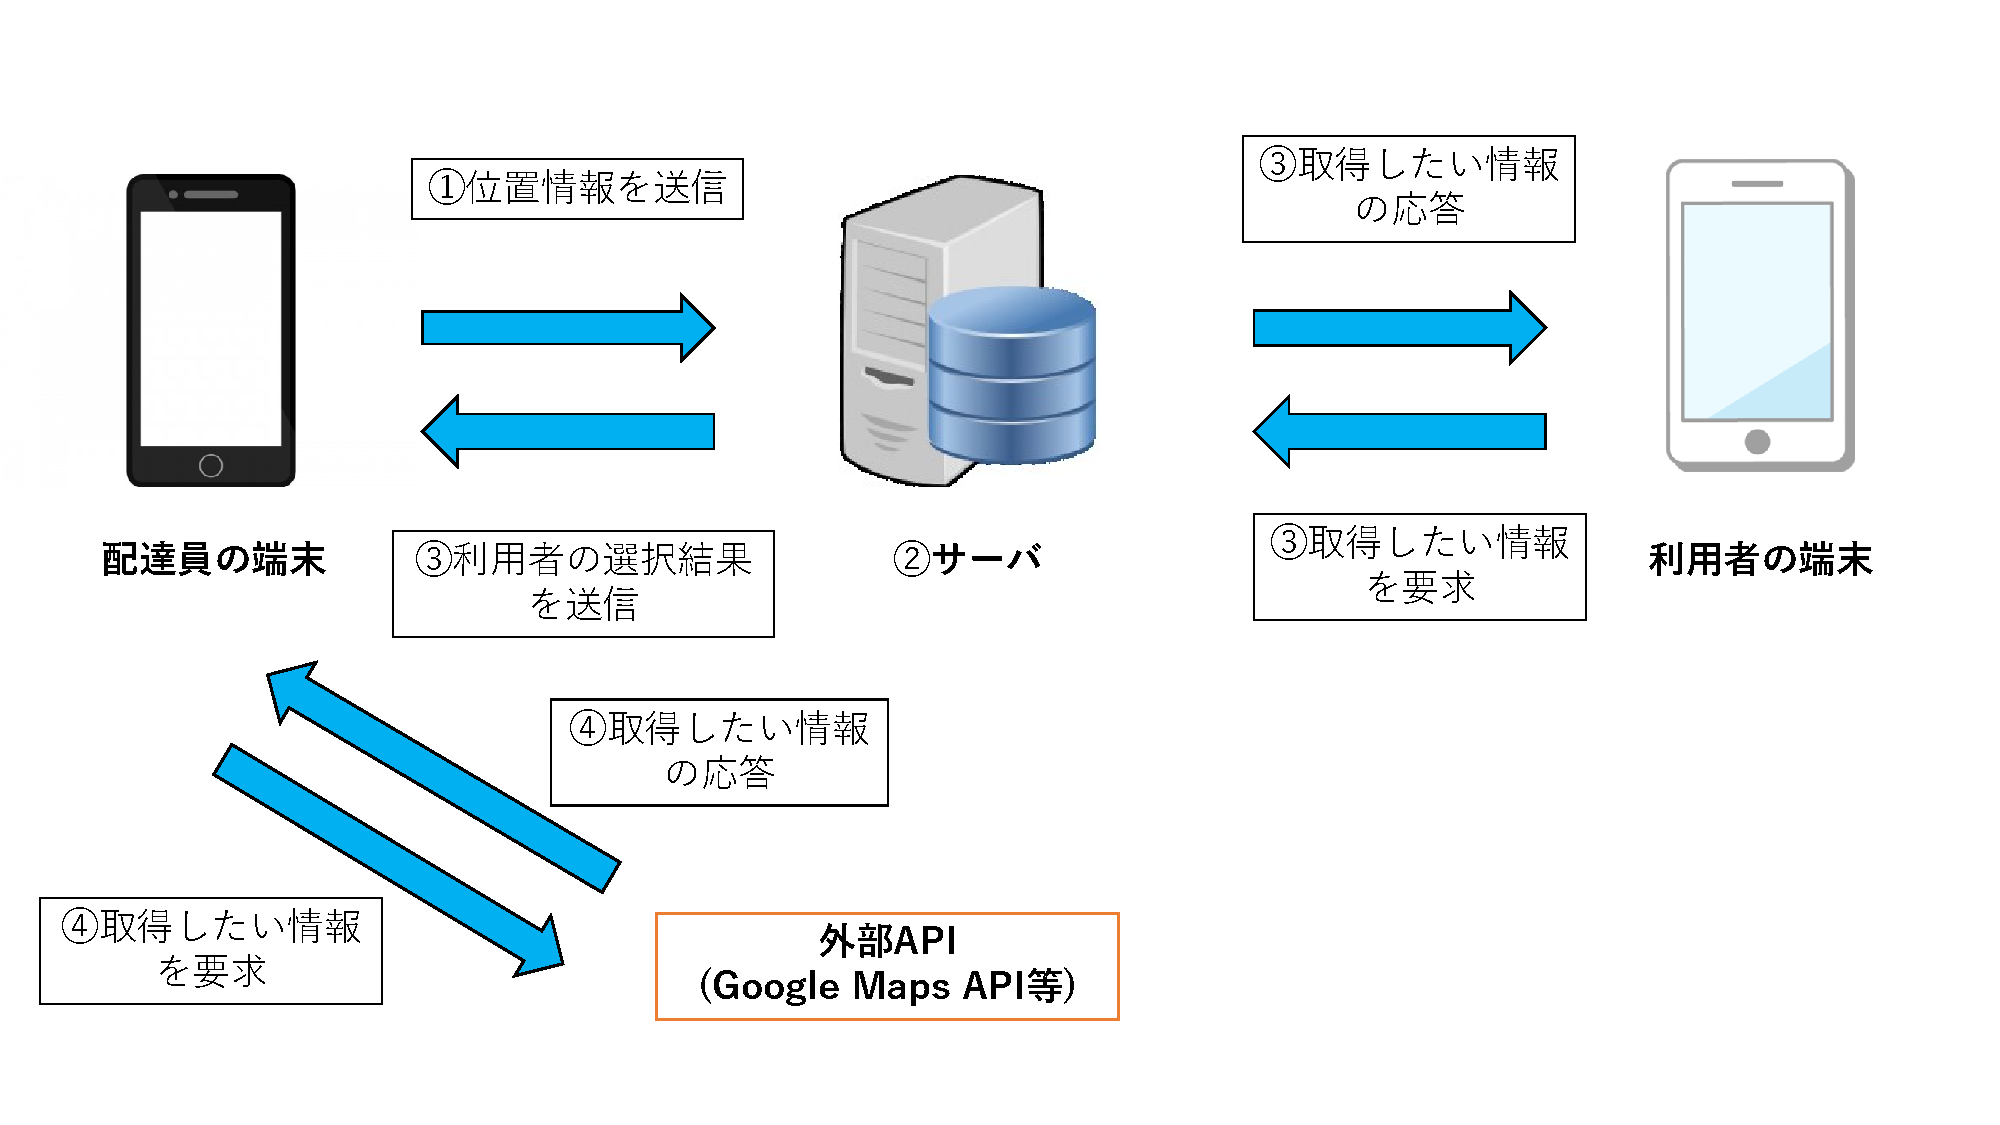
\includegraphics[width=140mm]{information_flow.pdf}
	\caption{ネットワーク構成}
	\label{fig:i_f}
 \end{center}

\end{figure}


\section{ネットワーク接続形態}
本システムでは利用者端末,管理者端末は TCP/IP を用いてサーバと通信を行います.


\section{用語の定義}
本システムでは以下のように用語を定義します.
\begin{itemize}
 \item 利用者:ネットショッピングなどを通じて商品を購入して,自宅に配送するように指定した消費者
 \item 配達員:宅配業者の従業員で商品をお客様の家まで届ける人
\end{itemize}

\begin{thebibliography}{9}

\bibitem{ref1}
国土交通省,
\newblock ``宅配便の再配達削減に向けて'',\\
\newblock \url{http://www.mlit.go.jp/seisakutokatsu/freight/re_delivery_reduce.html}, \\
2018/10/11
\bibitem{ref2}
エン・ジャパン株式会社,
\newblock ``ヤマト運輸株式会社 中部支社のドライバー ★平均月収35万円。無理なく年収400万円が見込めます。'',\\
\newblock \url{https://employment.en-japan.com/desc_770664/}, \\
2018/10/11
\end{thebibliography}

\end{document}
